\documentclass[11pt,border=6pt]{standalone}
\usepackage{fontspec}
\usepackage{tikz}
\usetikzlibrary{positioning,arrows.meta,calc}
\begin{document}
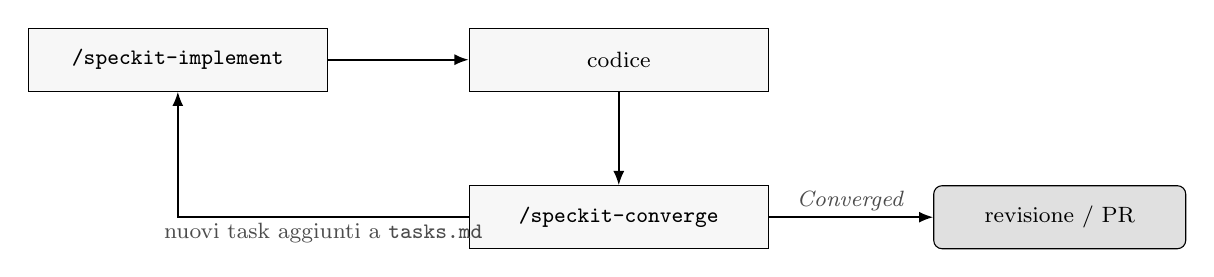
\begin{tikzpicture}[font=\footnotesize,
  cmdbox/.style={draw, minimum width=3.8cm, minimum height=8mm, align=center,
    fill=black!3, font=\footnotesize},
  resbox/.style={draw, rounded corners=3pt, minimum width=3.2cm, minimum height=8mm,
    align=center, fill=black!12, font=\footnotesize},
  arr/.style={-{Latex[length=1.8mm,width=1.4mm]}, semithick},
  lbl/.style={font=\footnotesize, text=black!70, inner sep=2pt}]

  \node[cmdbox] (impl) at (0,0) {\texttt{/speckit-implement}};
  \node[cmdbox] (code) at (5.6,0) {codice};
  \node[cmdbox] (conv) at (5.6,-2.0) {\texttt{/speckit-converge}};
  \node[resbox]  (pr)   at (11.2,-2.0) {revisione / PR};

  \draw[arr] (impl.east) -- (code.west);
  \draw[arr] (code.south) -- (conv.north);
  \draw[arr] (conv.west) -| node[lbl, below, pos=0.25] {nuovi task aggiunti a \texttt{tasks.md}} (impl.south);
  \draw[arr] (conv.east) -- node[lbl, above] {\emph{Converged}} (pr.west);
\end{tikzpicture}
\end{document}


